We have defined \textit{TinyFace} in the \textit{Introduction} as a face detector application, powered by neural networks and running in a TensorFlow-Lite interpreter, where certain steps have been undertaken to reduce the model size and complexity. This chapter will present a working application where this has been made possible.
\section{The Workflow}
We had to compile a Neural Network Model Architecture in Python, using Keras and then the TFLite libraries for optimization. The conversion part is especially important here, since it encompasses all the necessary TFLite model optimizations that we are undertaking to make a particular model meet the our size constraints. \par

\section{TinyFace}
Let us now present a working implementation of face detection. We have settled on the parameters and configuration presented below after experimenting with several datasets and many different model architectures. 
\subsection{A Model Architecture That Stands Apart}
The used neural network model is based on the \textit{SqueezeNet} architecture. SqueezeNet - which is a classification neural network - manages to achieve very small model sizes, because it uses \textit{concatenations} to merge layers. As such, the network is a sequence of convolutional and pooling layers, plus what its authors call \textit{fire modules} or layers, which use the above named convolutions. An overview of one fire layer can be seen in \textit{Table \ref{tab:fire_layer}}, and the complete architecture of the neural network can be seen in \textit{Table \ref{tab:optimized_squeezenet}}. \par
\subfile{figures/squeezenet}
Other models that the author has experimented with are VGG-3, LeNet and DarkNet, which were presented in the previous chapter. However, the size of these could not be reduced enough to make them fit on the embedded device. \par 
For determining the training parameters, the author experimented by gradually increasing the dimensions and definition of training data until either the performance started decreasing or the computer ran out of memory. For instance, trying to train with anything more than 50,000 color images with sides larger than 100 pixels, could not fit inside the video memory of the used graphics card, and resulted in an error.
\begin{figure}
    \centering
    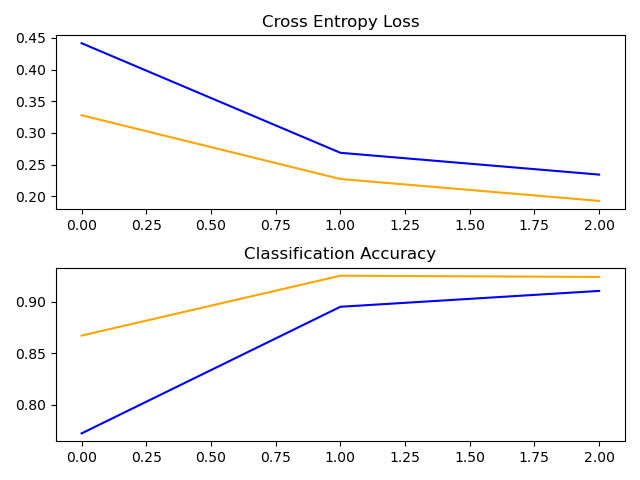
\includegraphics[height = 10 cm]{images/squeezenet_3epochs.png}
    \caption{Training the final version of the model. A squeezenet-based model architecture, with 3 epochs of training, and a batch size of 32, plus a custom dataset of 16,000 samples. This trained model run with acceptable accuracy in the webcam demo.}
    \label{fig:squeezenet_final_3_epochs}
\end{figure}
\subsection{Validation on a PC}
For quick validation, on the same device where training has been done, a computer application was built. This can save valuable time that would otherwise have been wasted deploying a model to the embedded hardware - especially since most models were far from accurate or small enough from the get-go. This app uses a local model interpreter, which can read \textit{.tflite} files and run inference from these locally. The app can take, as input, both static pictures and live webcam frame capture. It also runs in real-time. This offers very valuable feedback before deployment to the actual edge hardware.

